% vim:encoding=utf8 ft=tex sts=2 sw=2 et:

\documentclass{classrep}
\usepackage[utf8]{inputenc}
\usepackage[pdftex]{color,graphicx}
\DeclareGraphicsExtensions{.pdf,.png,.jpg}
\usepackage{float}
\usepackage{color}
\usepackage{listings}
\usepackage{color}
 \usepackage{hyperref}
\definecolor{dkgreen}{rgb}{0,0.6,0}
\definecolor{gray}{rgb}{0.5,0.5,0.5}
\definecolor{mauve}{rgb}{0.58,0,0.82}
\lstset{ %
  language=Matlab,                % the language of the code
  basicstyle=\footnotesize,           % the size of the fonts that are used for the code
  numbers=left,                   % where to put the line-numbers
  numberstyle=\tiny\color{gray},  % the style that is used for the line-numbers
  stepnumber=2,                   % the step between two line-numbers. If it's 1, each line 
                                  % will be numbered
  numbersep=5pt,                  % how far the line-numbers are from the code
  backgroundcolor=\color{white},      % choose the background color. You must add \usepackage{color}
  showspaces=false,               % show spaces adding particular underscores
  showstringspaces=false,         % underline spaces within strings
  showtabs=false,                 % show tabs within strings adding particular underscores
  frame=single,                   % adds a frame around the code
  rulecolor=\color{black},        % if not set, the frame-color may be changed on line-breaks within not-black text (e.g. commens (green here))
  tabsize=2,                      % sets default tabsize to 2 spaces
  captionpos=b,                   % sets the caption-position to bottom
  breaklines=true,                % sets automatic line breaking
  breakatwhitespace=false,        % sets if automatic breaks should only happen at whitespace
  title=\lstname,                   % show the filename of files included with \lstinputlisting;
                                  % also try caption instead of title
  keywordstyle=\color{blue},          % keyword style
  commentstyle=\color{dkgreen},       % comment style
  stringstyle=\color{mauve},         % string literal style
  escapeinside={\%*}{*)},            % if you want to add a comment within your co
}


\studycycle{Informatyka, studia dzienne, mgr II st.}
\coursesemester{I}

%\coursename{Angelologia teoretyczna i stosowana}
\coursename{Metody obliczeniowe optymalizacji}
\courseyear{2011/2012}

\courseteacher{Prowadzący}
\coursegroup{dzień, godzina}

\author{
  \studentinfo{Paweł Musiał}{nr albumu 1} \and
  \studentinfo{Łukasz Michalski}{nr albumu 2}
}

\title{1: Optymalizacja jednowymiarowa} % np \title{Zadanie 1: Optymalizacja jednowymiarowa}
\svnurl{http://serce.ics.p.lodz.pl/svn/labs/moo/adres@rewizja}

\begin{document}
\maketitle

\section{Cel}
Zaimplementować 3 metody optymalizacji jednowymiarowej spośród następujących:
\begin{itemize}
	\item	metoda dychotomii
	\item	\textbf{metoda bisekcji}
	\item	metoda złotego podziału
	\item	\textbf{metoda Fibonacci}
	\item	metoda Newtona
	\item	\textbf{metoda Quasi-Newtona}
\end{itemize}
Przedstawiany jako rozwiązanie program powinien pozwolić wprowadzić funkcję oraz przedział, w którym poszukiwane będzie rozwiązanie. Jeśli przedział nie jest unimodalny należy wyznaczyć przedział unimodalności. Skonfrontować wyniki z wyznaczonymi za pomocą pakietu Matlab. Porównać efektywność zaimplementowanych metod.
\section{Rozwiązanie zadania}

\subsection{Wyznaczanie podprzedziału unimodalności}
Wyznaczanie podprzedziału unimodalności jest wykonywane poprzez sprawdzanie kolejnych podprzedziałów o określonej szerokości. W każdym takim podprzedziale sprawdzana jest lokalna unimodalność funkcji. Gdy znajdziemy podprzedział który spełnia te kryteria zwracamy go jako nowy podprzedział do poszukiwania rozwiązania. Każdorazowe wyszukiwanie, podprzedziału unimodalności nie tylko sprawdza czy funkcja jest lokalnie unimodalna, lecz również zmniejsza zakres poszukiwań rozwiązania.
\subsection{Metoda bisekcji \cite{1}}
Metoda ta polega na wybraniu trzech punktów jednakowo odległych od siebie oraz od krańców przedziału oraz wyliczeniu wartości funkcji w tych punktach, w wyniku czego można wyeliminować połowę przedziału.\\
Algorytm\\
\begin{enumerate}

\item Wybierz dolne i górne ograniczenie przedziału a i b oraz małą liczbę $\epsilon$. Niech $x_m = (a + b)/2$, $L_0 =L=b-a$. Wylicz $f(x_m )$.
\item Ustal $x_1 = a + L/4$, $x_2 = b - L/4$. Wylicz $f(x_1 )$ oraz $f(x_2 )$.
\item Jeśli $f(x_1 ) < f(x_m )$, ustal $b = x_m$ ; $x_m = x_1$ ; Przejdź do 5);\\
 W przeciwnym wypadku przejdź do kroku 4).
\item Jeśli $f(x_2 ) < f(x_m )$, ustal $a = x_m$ ; $x_m = x_2$ ;\\
 W przeciwnym przypadku ustal $a = x_1$ , $b = x_2$ ;
\item Wylicz $L = b - a$. Jeśli $|L| < \epsilon$, Zakończ;\\
 W przeciwnym przypadku przejdź do 2).
\end{enumerate}
 \\

\indent W każdej nowej iteracji algorytmu, potrzebne jest wyliczenie dwóch wartości funkcji, a przedział zmniejsza się o połowę. Po n-krotnym wyliczeniu wartości funkcji, przedział zmniejsza się do około $0.5^{n/2} L_0$ . Czyli ilość razy n, ile trzeba policzyć wartości funkcji, aby osiągnąć daną dokładność $\epsilon$ można policzyć z następującego wzoru : 
$$(0.5)^{n/2} (b - a) = \epsilon$$


\subsection{Metoda Fibonacci \cite{1}}
W metodzie liczb Fibonacciego, w każdej iteracji algorytmu proporcja zmniejszania się przedziału z iteracji na iterację zmienia się tak, aby przedział zmniejszał się w sposób optymalny (tzn. jak najbardziej). Jeśli $p_k$ oznacza proporcje, o jaką zmniejsza się przedział w k-tej iteracji, to w metodzie Fibonacciego zachodzi następujący związek:\\
$$\frac{1-p_{k-1}}{1} = \frac{p_k}{1-p_k}$$
Okazuje się, że wartościami $p_k \in (0, 1/2]$, gdzie k = 1,..., N, które minimalizują wyrażenie $(1-p_1)(1-p_2)...(1-p_N)$ i które spełniają powyższy związek, są następujące liczby:
$$p_k=1-\frac{F_{N-k-1}}{F_{N-k+2}} $$
gdzie $F_k$ oznaczają liczby Fibonacciego. Liczby Fibonacciego mają następującą charakterystykę: $F_1 = 1, F_2 = 1$ i $F_k = F_{k−1} + F_{k−2}$ gdzie k = 3, 4, ....\\

Algorytm\\
\begin{enumerate}
\item Znajdź n takie, że $\frac{(b-a)}{F_n}\geq 2\epsilon$
\item Oblicz $x_1 = \frac{F_{n-1}}{F_n}(b-a)$ i $x_2 = \frac{F_{n-1}}{F_n}(b-a)$
\item  Jeżeli $f(x_1)<f(x_2)$ to podstaw :
	\begin{itemize}
	\item $b=x_2$
	\item $x_2=x_1$
	\item $n=n-1$
	\item $x_1 = b - \frac{F_{n-1}}{F_n}(b-a)$
	\end{itemize}
	\\
	W przeciwnym wypadku :
	\begin{itemize}
	\item $a=x_1$
	\item $x_1=x_2$
	\item $n=n-1$
	\item $x_2 = a + \frac{F_{n-1}}{F_n}(b-a)$
	\end{itemize}	
	\item Jeśli $|x_2-x_1|>\epsilon$ i $n \geq 2$ przejdź do 3.
\end{enumerate}
\\

W tym algorytmie przedział redukuje się do $\frac{2}{F_{N+1}} L$ do czego potrzebnych jest n wyliczeń wartości funkcji. Zatem ilość potrzebnych wyliczeń wartości funkcji przy danej dokładności $\epsilon$ można wyliczyć z następującego wzoru:\\
$$\frac{2}{F_{n+1}} = \epsilon$$
Jednym z minusów metody liczb Fibonacciego jest fakt, iż trzeba wyliczać kolejne liczby Fibonacciego w każdej iteracji.

\subsection{Metoda Quasi-Newtona}
Metody quasi-Newtonowskie bazują na metodzie Newtona znajdowania punktów stacjonarnych funkcji. Metoda Newtona zakłada, że funkcja może być lokalnie aproksymowana funkcją kwadratową w otoczeniu optimum, oraz używają pierwszych i drugich pochodnych (gradient i hesjan) w celu znalezienia punktów stacjonarnych.\\
W metodzie Quasi-Newtona hesjan(macierz drugich pochodnych) minimalizowanej funkcji nie musi być obliczany. Hesjan jest przybliżany przez analizowanie kolejnych wektorów gradientu. Metody Quasi-Newtona są uogólnieniem metody siecznych znajdowania pierwiastków pierwszej pochodnej na problem wielowymiarowy.\\
Kolejne przybliżenia są wyznaczane na podstawie :\\
\begin{equation}
x_{k+1} = x_k - \frac{x^k-x^{k-1}}{f'(x^k)-f'(x_{k-1})} f'(x_k)
\end{equation}

\section{Opis programu}

Program składa się z implementacji 3 wyznaczonych metod, oraz funkcji pomocniczych do określania podprzedziału unimodalności i rysowania wykresu funkcji z nałożonymi punktami kolejnych przybliżeń rozwiązania.

\subsection{Wyznaczanie podprzedziału unimodalności}
\begin{lstlisting}
function [a, b] = unimodality_check(f,a,b, step)

unimodal=0;
a=a+step;

while unimodal==0 && a<b
    %found max || min
    if (feval(f,a-step) < feval(f,a) &&
     feval(f,a+step) < feval(f,a)) ||
      (feval(f,a-step) > feval(f,a)
       && feval(f,a+step) > feval(f,a))
        unimodal=1;
    else
        a=a+step;
    end
end

if unimodal == 0
    disp('przy danym kroku probkowania,
     nie znaleziono podprzedzialu unimodalnosci');
    a=-1;b=-1; 
elseif unimodal == 1
    b=a+step;
end
\end{lstlisting}

\subsection{Metoda bisekcji}
\begin{lstlisting}
function [c,yc,iter] = bisection (f,a,b,eps)
f=inline(f);
xL=a;xR=b;
maxIterations=5+round((log(a-b)-log(eps))/log(2));

while ( abs(xR - xL) > eps && i< maxIterations)
    c=(xL+xR)/2.0;
    yc=feval(f,c);
    l=xR-xL;
    x1=xL+(l/4.0);
    x2=xR-(l/4.0);
    if feval(f,x1)<feval(f,c)
        xR=c;
        c=x1;
    elseif feval(f,x2)<feval(f,c)
        xL=c;
        c=x2;
    else
        xL=x1;
        xR=x2;
    end
    i=i+1
end
\end{lstlisting}


\section{Metoda Fibonacciego}
\begin{lstlisting}

function x = fib(n)
if n<=0
    x=0;
elseif n==1
    x=1;
else x=fib(n-1)+fib(n-2);
end


function [c,yc,iter] = fibonaccio (f,a,b,eps)
f=inline(f);
n=0;
while 1.0/fib(n) > eps
    n=n+1;
end

x1=b-(fib(n-1)/fib(n))*(b-a);
x2=a+(fib(n-1)/fib(n))*(b-a);

while ( abs(x2 - x1) > eps && n >= 2)
    c=(a+b)/2;
    yc=feval(f,c);
    if feval(f,x1)<feval(f,x2)
        b=x2;
        x2=x1;
        n=n-1;
        x1=b-(fib(n-1)/fib(n))*(b-a);
    else
        a=x1;
        x1=x2;
        n=n-1;
        x2=a+(fib(n-1)/fib(n))*(b-a);
    end
end

c=(a+b)/2;
yc=feval(f,c);
\end{lstlisting}


\subsection{Metoda Quasi-Newtona}


\begin{lstlisting}

function [b,by,k]=quasi_newton(f,a,b,eps)
f=inline(f);

maxIterations=5+round((log(a-b)-log(eps))/log(2));

k=1;
while  k < maxIterations    
    p2=b-diffp(f,b)*(b-a)/(diffp(f,b)-diffp(f,a));    
    err=abs(p2-b);
    a=b;
    b=p2;
    by=feval(f,b);
    if (err<eps)
        break
    end
   k=k+1; 
end

function var = diffp (f,p)
var=feval(inline(diff(sym(f))),p);
\end{lstlisting}

\section{Wyniki}
	\begin{table}[H]
		\begin{center}
\begin{tabular}{|c|c|c|c|c|c|c|c|}

\hline funkcja & metoda & xs & xk & eps & xmin & ymin & iter \\
\hline $x^2 - 4$ & bisekcja & -1 & 3 & 0.1 & 0.0313 & -3.9961 & 4\\
\hline $x^2 - 4$ & bisekcja & -1 & 3 & 0.01 & 0.0039 & -3.9999 & 7\\
\hline $x^2 - 4$ & bisekcja & -1 & 3 & 0.001 & 4.8828e-004 & -4.0000 & 10 \\
\hline $x^2 - 4$ & fibonacci & -1 & 3 & 0.01 & 0.0174 & -3.9997 & 7\\
\hline $x^2 - 4$ & fibonacci & -1 & 3 & 0.001 & 0.0016 & -4.0000 & 12 \\
\hline $x^2 - 4$ & quasi-newton & -1 & 3 & 0.001 & 0 & -4 & 2\\
\hline $-x + x^2 - 3*x^3 + x^4$ & bisekcja & -1 & 3 & 0.1 & 2.0625 & -6.0339 & 4 \\
\hline $-x + x^2 - 3*x^3 + x^4$ & bisekcja & -1 & 3 & 0.01 & 2.0664 & -6.0339 & 7 \\
\hline $-x + x^2 - 3*x^3 + x^4$ & bisekcja & -1 & 3 & 0.001 & 2.0664 & -6.0341 &10 \\
\hline $-x + x^2 - 3*x^3 + x^4$ & fibonacci & -1 & 3 & 0.01 & 2.0729 & -6.0337 & 7 \\
\hline $-x + x^2 - 3*x^3 + x^4$ & fibonacci & -1 & 3 & 0.001 & 2.0673 & -6.0341 & 12 \\
\hline $-x + x^2 - 3*x^3 + x^4$ & quasi-newton & -1 & 3 & 0.001 & 2.0666 & -6.0341 & 4\\
\hline $sin(x)+x-x^3$ & bisekcja & -15 & 15 & 0.01 & -0.7578 & -1.0100 & 7\\
\hline $sin(x)+x-x^3$ & bisekcja & -15 & 15 & 0.001 & -0.7583 & -1.0100 & 10\\
\hline $sin(x)+x-x^3$ & fibonacci & -15 & 15 & 0.01 & -0.7604 & -1.0099 & 7 \\
\hline $sin(x)+x-x^3$ & fibonacci & -15 & 15 & 0.001 & -0.7592 & -1.0099 & 12\\
\hline $sin(x)+x-x^3$ & quasi-newton & -15 & 15 & 0.001 & -0.7585 & -1.0100 & 6 \\
\hline $x^3*arctan(x)-exp(x)$ & bisekcja & -1 & 3 & 0.01 & 1.0039 & -1.9317 & 7 \\
\hline $x^3*arctan(x)-exp(x)$ & bisekcja & -1 & 3 & 0.001 & 1.0005 & -1.9327 & 10\\
\hline $x^3*arctan(x)-exp(x)$ & fibonacci & -1 & 3 & 0.001 & 1.0016 & -1.9327  & 12\\
\hline $x^3*arctan(x)-exp(x)$ & quasi-newton & -1 & 3 & 0.001 & 0.9685 & -1.9350 & 4 \\
\hline
\end{tabular} 
				\caption{Zestawienie wyników z badań metod.}
		\end{center}
	\end{table}
	
	\begin{figure}[H]
  \centering
    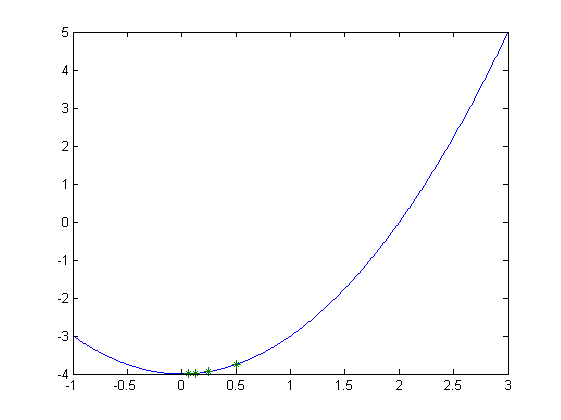
\includegraphics[width=0.8\textwidth]{b_eps01}
	 \caption{Przykład graficzny kolejnych przybliżeń w metodzie bisekcji.}
 \end{figure}
 \begin{figure}[H]
  \centering
    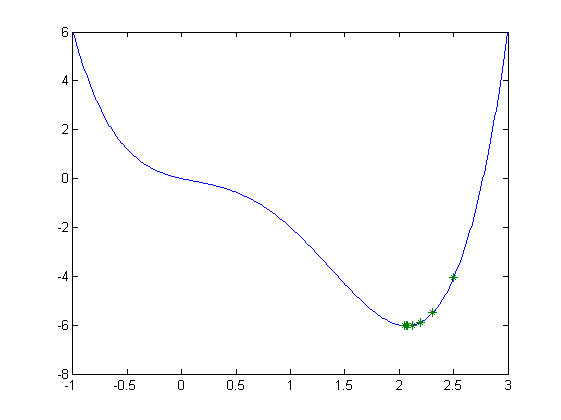
\includegraphics[width=0.8\textwidth]{f_eps001}
	 \caption{Przykład graficzny kolejnych przybliżeń w metodzie liczb Fibonacciego.}
 \end{figure}
 \begin{figure}[H]
  \centering
    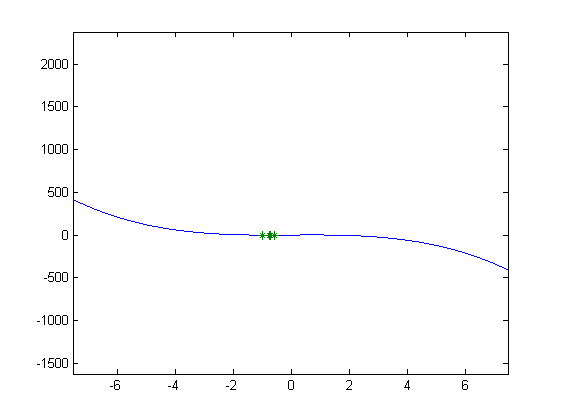
\includegraphics[width=0.8\textwidth]{q_eps0001}
	 \caption{Przykład graficzny kolejnych przybliżeń w metodzie Quasi-newtona.}
 \end{figure}
 
 	\begin{table}[H]
		\begin{center}
		\begin{tabular}{|c|c|c|}
		\hline funkcja & x & y \\ 
\hline $x^2 - 4$ & -4 & 0 \\ 
\hline $-x + x^2 - 3*x^3 + x^4$ \footnote{lokalne minimum} & 2.06659 & -6.03405 \\ 
\hline $sin(x)+x-x^3$ \footnote{lokalne minimum} & -0.758481 & -1.00995 \\ 
\hline $x^3*arctan(x)-exp(x)$ \footnote{lokalne minimum} & 0.968539 & -1.93503 \\ 
\hline 
\end{tabular} 
				\caption{Zestawienie wyników uzyskanych przy pomocy WolframAlpha\footnote{\url{www,wolframalpha.com}}}.
		\end{center}
		\label{wolfram}
	\end{table}
	

\section{Wnioski}

Na podstawie wykonanych badań, można stwierdzić, że metoda Quasi-newtona, osiąga najlepsze wyniki odnosząc się do wyników zestawionych w tabeli \ref{wolfram}. Równocześnie nie tylko najdokładniejsza ale również najszybsza w działaniu. W każdym przypadku zadaną dokładność osiągała po około połowie iteracji których potrzebowały metody Fibonacciego i bisekcji. 


\begin{thebibliography}{0}
\item
  Michał Lewandowski,
  \emph{Metody optymalizacji - teoria i wybrane algorytmy}.
  2012.
  
\item \url{http://pl.wikipedia.org/wiki/Metoda_quasi-Newtona}
\end{thebibliography}

\end{document}
